\documentclass{llncs}
\usepackage[T2A]{fontenc}
\usepackage[utf8]{inputenc}
\usepackage[russian]{babel} 
\usepackage{graphicx}
\usepackage{natbib}
\usepackage{amsfonts}
\usepackage{alltt}


\title{Распознавание текста на основе скелетного представления толстых линий и сверточных сетей }

\author{Тушин К.А.}
\institute{Московский физико-технический институт (Государственный университет) \\ \email{tushin.ka@phystech.edu}}

\begin{document}

\maketitle

\begin{abstract}
В работе рассматриваются подходы решения задачи распознования символов. Один из методов используюет сверточные сети для классификации изображений. Другой метод заключается в анализе графовых струтур с помощью скелетного представления, полученных по изображению. Так же приведены сравнения точности этих подходов и архитектур на датасетах MNIST.
\end{abstract}

\textit{Ключевые слова: сверточные нейронные сети, CNN, распознавание символов, скелетное представление, Graph embedding}

\section{Введение}
Распознования символов это классическая задача компьютерного зрения. Основным подходом в таких задачах это использование сверточных слоев в нейросетях~\cite{cnn_lecun}~\cite{cnn_appl}. В таких нейросетях на вход подается изображение а на выходе получаем вероятность принадлежности изображения к каждому классу. Существует другой подход, при котором растровое изображение переводится в векторное представление путем построения скелета символа, а потом подается на вход модели для предсказания к какому классу принадлежит изображение.

Скелетизация представляет собой процесс заполнения внутренностей символов кругами, центры которых - вершины графа, соединяются с ребрами графа. Было проведено много много исследований на эту тему. В работе~\cite{graphs_gen} обсуждается моделирование рукописного текста с помощью жирных линий. В работе~\cite{graphs_shape_comp} проводится сравнение формы бинарных растровых изображений на основе скелетизации. Однако, существует и альтернативные методы, как, например описанный в работе~\cite{graphs_alt_method}. В этой работе главной задачей было распрямление текстовых строк на основе непрерывного гранично-скелетного представления изображений. 

Для оценки качества работы алгоритма использовалась метрика accuracy
на датасете, MNIST.

\section{Постановка задачи}

Введём следующие обозначения:

\item $\mathbb{A}$ - алфавит.
\item $\mathbb{I}$ - множество изображений c символами из $\mathbb{A}$.
\item $f: \mathbb{I} \rightarrow \mathbb{A}$ - функция сопостовляющая каждому элементу из $\mathbb{I}$ элемент из $\mathbb{A}$.
\item $\mathbb{S}$ - множество скелетных представлений символов на изображении из $\mathbb{I}$.
\item $a_1: \mathbb{I} \rightarrow \mathbb{S}$ - функция сопостовляющая каждому элементу из $\mathbb{I}$ скелетное представление из $\mathbb{S}$.
\item $\mathbb{F}$ - множество наборов признаков скелетных представлений из $\mathbb{S}$.
\item $a_2: \mathbb{S} \rightarrow \mathbb{F}$ - функция однозначно сопоставляющая скелетному представлению из $\mathbb{S}$ набор признаков из $\mathbb{S}$. 

Тогда задачей будет построить такую функцию $a_3: \mathbb{F} \rightarrow \mathbb{A}$, чтобы минимизировать функцию потерь - функция кросс энтропии на выборке изображений $\mathbb{I}$.

\section{Описание базовых алгоритмов}
\subsection{Неронная сеть}
В качестве первого базового алгоритма было решено использовать нейронную сеть с использованием сверточных слоев. 
\begin{alltt}
model = Sequential()
model.add(Conv2D(32, (3, 3),
                 activation='relu',
                 input_shape=(28,28,1))
model.add(Conv2D(64, (3, 3), activation='relu'))
model.add(MaxPooling2D(pool_size=(2, 2)))
model.add(Dropout(0.25))
model.add(Flatten())
model.add(Dense(128, activation='relu'))
model.add(Dropout(0.5))
model.add(Dense(10, activation='softmax'))

model.compile(loss="categorical_crossentropy",
              optimizer="adam",
              metrics=['accuracy'])
\end{alltt}
\subsection{Градиентный бустинг}
В качестве второй базовой модели использовался LightGBM classifier обученный на признаках из скелетного представления. Данный алгоритм основывается на градиентном бустинге над деревьями решений. Данный алгоритм показал наилучшие результаты на датасете MNIST. Используемые параметры модели : 
\begin{alltt}
model = LGBMClassifier(boosting_type='gbdt', num_leaves=31, 
max_depth=-1,learning_rate=0.1,n_estimators=100, 
subsample_for_bin=200000, objective=None, class_weight=None, 
min_split_gain=0.0,min_child_weight=0.001, min_child_samples=20,
subsample=1.0, subsample_freq=1, colsample_bytree=1.0,reg_alpha=0.0,
reg_lambda=0.0,random_state=None, n_jobs=-1, silent=True)
\end{alltt}


\section{Планирование эксперимента}
\subsection{Неронная сеть}
Модель на вход принимала черно-белые изображения размером 28 на 28. На выходе получали вероятности принадлежности к каждому из классов. При обучении уменьшался learning rate в два раза, каждый раз когда модель не улучшала на валидации метрику в течении трех эпох. И прекращалось обучение, если в течении 5 эпох не улучшалось значение метрики.
\subsection{Градиентный бустинг}
Для того, чтобы построить скелет, картинку необходимо было бинаризовать. В этих данных бинаризация была следующая: все пиксели, цвет которых НЕ черный (то есть > 0 в нотации цветов от 0 до 255), становятся белыми. 
На каждую картинку в выборке отводится массив из чисел: каждые 8 подряд идущих чисел описывают ребро скелета: по 4 числа на каждую вершину ребра: (xcoord, ycoord, deg, rad), (xcoord, ycoord) — координаты вершины, deg — степень вершины (она может быть от 1 до 3, таков алгоритм построения скелета), rad — радиальная функция в этой точке, или же, радиус вписанной в фигуру окружности в этой точке.

На вход модель принимала различного рода статистики, посчитанные на скелетном представлении изображения.
Используемые статистики:
\begin{itemize}
    \item Количество вершин в скелетном представлении
    \item Среднее значение среди всех чисел, как представленных в описании графа, так и по каждой из 8 подряд идущих чисел
    \item Сумма как всех чисел, представленных в описании графа, так и по каждой из 8 подряд идущих чисел
    \item Дисперсия как среди всех чисел, представленных в описании графа, так и по каждой из 8 подряд идущих чисел
    \item Разность между максимальным и минимальным числом как среди всех чисел, представленных в описании графа, так и по каждой из 8 подряд идущих чисел
    \item Перцентили от 0 до 1 с шагом 0.1 как среди всех чисел, представленных в описании графа, так и по каждой из 8 подряд идущих чисел
    \item Для каждой из четырёх категорий самое частое значение и сколько раз оно встретилось
\end{itemize}

\section{Анализ ошибки}

\begin{wrapfigure}
\centering
\caption{Анализ функции ошибки нейросети\label{overflow}}
\begin{center}
    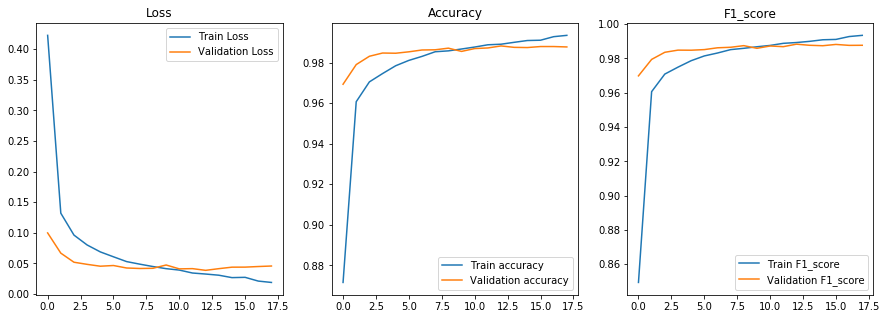
\includegraphics[width=90mm]{loss.jpg}
  \end{center}
\end{wrapfigure}
На графиках представленны изменения ошибки и значений метрики в зависимости от количества эпох в обучении нейронной сети. Видно что модель быстро сходится к минимумум ошибки.

\section{Анализ структуры модели}
\subsection{Неронная сеть}
Добавление других слоев в модель практически не меняло качество модели, поэтому не изменялась архитектура модели от базовой модели. Поэтому архитектура модели выглядит следующим образом:

\begin{wrapfigure}
\centering
\caption{Структура нейронной сети\label{overflow}}
\begin{center}
    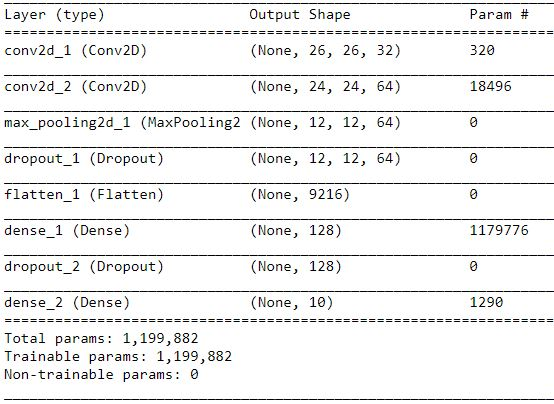
\includegraphics[width=90mm]{model.jpg}
  \end{center}
\end{wrapfigure}

\subsection{Градиентный бустинг}
После построения признаков были проведенны эксперименты по изменению параметров модели. Наилучшими признаками оказались признаки по умолчанию.

\section{Выбор модели}
После того как были проведенны эксперименты, полученные признаки из скелетного представления были добавлены в модель нейронной сети и проведен еще один эксперимент.
В таблице представлена таблица сравнения результатов моделей на тестовой выборке.

\begin{wraptable}
\label{tabular:timesandtenses}
\begin{center}
\begin{tabular}{ccc}
Модель & Accuracy & F1-score \\
LightGBM: & \textbf{0.9314} & \textbf{0.9304} \\
Нейросеть: & \textbf{0.9882} & \textbf{0.9883} \\
Нейросеть + features & \textbf{0.9864} & \textbf{0.9867} \\
\end{tabular}
\end{center}
\end{wraptable}

\section{Результат работы}
В результате работы было рассматренно несколько подходов к решению задачи распознования символов. Один из методов использовал сверточные сети для классификации изображений. Другой метод заключался в анализе графовых струтур с помощью скелетного представления, полученных по изображению. Так же были приведены сравнения точности этих подходов и архитектур на датасетах MNIST.

\begin{thebibliography}{1}

\bibitem{cnn_lecun}
	\BibAuthor{LeCun Y. et al.}
	 Convolutional networks for images, speech, and time series //The handbook of brain theory and neural networks. – 1995. – Т. 3361. – №. 10. – С. 1995.
	 
\bibitem{cnn_appl}
	\BibAuthor{Ciresan D. C. et al.}
 	Convolutional neural network committees for handwritten character classification //Document Analysis and Recognition (ICDAR), 2011 International Conference on. – IEEE, 2011. – С. 1135-1139.
 
\bibitem{graphs_gen}
	\BibAuthor{Клименко С. В., Местецкий Л. М., Семенов А. Б.}
	 Моделирование рукописного шрифта с помощью жирных линий //Труды. – 2006. – Т. 16.

\bibitem{graphs_shape_comp}
	\BibAuthor{Кушнир О. и др.}
	 Сравнение формы бинарных растровых изображений на основе скелетизации //Машинное обучение и анализ данных. – 2012. – Т. 1. – №. 3. – С. 255-263.
	 
\bibitem{graphs_alt_method}
	\BibAuthor{Масалович А., Местецкий Л.}
	 Распрямление текстовых строк на основе непрерывного гранично-скелетного представления изображений //Труды Международной конференции «Графикон», Новосибирск.–2006.–4 c.

\bibitem{mnist_original}
	\BibAuthor{LeCun Y., Cortes C., Burges C. J.}
	MNIST handwritten digit database //
	Available: 
	 \BibUrl{http://yann. lecun. com/exdb/mnist}. – 2010. – Т. 2.

\bibitem{mnist_sample1}
	\BibAuthor{Zhu D. et al.}
	 Negative Log Likelihood Ratio Loss for Deep Neural Network Classification //arXiv preprint arXiv:1804.10690. – 2018.
	 
\bibitem{mnist_sample2}
	\BibAuthor{Nair P., Doshi R., Keselj S.}
	Pushing the limits of capsule networks //Technical note. – 2018.

\bibitem{mnist_sample3}
	\BibAuthor{Hsieh P. C., Chen C. P.}
	 Multi-task Learning on MNIST Image Datasets. – 2018.

\end{thebibliography}

\end{document}

